% Fonts + Colors ~~~~

\usepackage{lipsum}
\usepackage{fontspec}
\usepackage{dashrule}
\usepackage[export]{adjustbox}
\usepackage[usenames, dvipsnames]{color}
\usepackage{comment}

\definecolor{Gray}{RGB}{120, 120, 120}
\definecolor{LogoRed}{RGB}{153, 0, 0}
\definecolor{LogoTurquoise1}{RGB}{1, 123, 147}
\definecolor{LogoTurquoise2}{RGB}{0, 158, 171}
\definecolor{LogoTurquoise3}{RGB}{0, 186, 187}
\definecolor{BackgroundBlue}{RGB}{247, 254, 255}
\definecolor{LightBlue}{RGB}{230, 247, 255}
\definecolor{LightRed}{RGB}{231, 103, 97}
\definecolor{DarkGray}{RGB}{71, 71, 71}

\begin{comment}
\newfontfamily\Avenir[
    Path= fonts/,
    Extension= .otf,
    UprightFont = *-45Book,
    ItalicFont = *-45BookOblique,
    BoldFont = *-95Black,
]{AvenirLTStd}

\newfontfamily\TradeGothic[
    Path = fonts/,
    Extension = .otf,
    UprightFont = *-No18,
    BoldFont = *-No20Bold,
]{TradeGothicCondensed}

\setmainfont[Ligatures=TeX]{Avenir}
\Avenir\fontsize{9pt}{12pt}\selectfont

\end{comment}

\usepackage[condensed]{roboto}
\usepackage[default,osfigures,scale=0.95]{opensans}
\usepackage[T1]{fontenc}

\fontsize{9pt}{12pt}\selectfont

% Formatting ~~~~

\usepackage{geometry}

\geometry{
    letterpaper,
    top=1.75in,
    bottom=1.75in,
    inner=0.75in,
    outer=0.75in,
    headsep=1in,
    headheight=0.5in,
    footskip=1in,
    % showframe
}

\usepackage[document]{ragged2e}
\parskip=8pt
\parindent=0pt
\linespread{1.2}
\setlength{\columnsep}{0.75cm}

% \usepackage{sectsty}
% \sectionfont{\fontfamily{pag}\selectfont\color{LogoTurquoise1}\vspace{-\parskip}\Large\uppercase}
% \subsectionfont{\color{LogoTurquoise1}\vspace{-\parskip}\mdseries\Large}

\usepackage{titlesec}
\titleformat*{\section}{\fontfamily{pag}\selectfont\color{LogoTurquoise1}\vspace{-\parskip}\bfseries\Large\uppercase}
\titleformat*{\subsection}{\color{LogoTurquoise1}\vspace{-\parskip}\Large}


% Headers + Footers ~~~~

\usepackage{fancyhdr}
\pagestyle{fancy}

\renewcommand{\sectionmark}[1]{\markboth{#1}{}}
\usepackage{fourier-orns}

\fancyhead{} % clear all header fields
\fancyfoot{} % clear all footer fields
\fancyfoot[LE]{\thepage \hspace{0.4cm} \roboto\selectfont\textcolor{LightRed}{\uppercase{Recruiting the Out-of-State University}}}
\fancyfoot[RO]{\roboto\selectfont\textcolor{Gray}{\leftmark} \hspace{0.4cm} \thepage}
\renewcommand{\headrulewidth}{0pt}

\fancypagestyle{tablepage}{  % No Header, Regular Footer
    \fancyhead{}
    \fancyfoot{}
    \renewcommand\headrule{\hrulefill
\raisebox{-2.1pt}[10pt][10pt]{\quad\decofourleft\decotwo\decofourright\quad}\hrulefill}
}

\addtolength{\skip\footins}{10pt}


% Links + Lists ~~~~

\PassOptionsToPackage{hyphens}{url}\usepackage[colorlinks=true, linkcolor=cyan, urlcolor=blue, citecolor=blue, breaklinks=true]{hyperref}
\newcommand{\superscript}[1]{$^{#1}$}

%reference list stuff
\usepackage[natbibapa]{apacite}

%\usepackage[super,numbers]{natbib}

\makeatletter
\renewcommand\@biblabel[1]{\superscript{#1}}
\makeatother

\renewcommand{\refname}{\vspace{-0.65cm}}

\usepackage{enumitem}
\setlist{nosep, itemsep=0pt, parsep=0pt, before={\large\color{DarkGray}}}

\renewcommand{\labelitemi}{\color{LightRed}$\triangleright$}
\renewcommand{\labelitemii}{\color{LogoTurquoise2}$\cdot$}
\renewcommand\labelitemiii{$\circ$}


% Block Formats ~~~~

\usepackage{mdframed}

\newenvironment{quote-block}{  % quote block
    \begin{quote}
    \roboto\selectfont
    \color{LogoTurquoise2}
}
{
    \end{quote}
}

\newenvironment{color-block}[1][Key Points]{  % text block
    \vspace{0.5cm}
    \begin{mdframed}[backgroundcolor=LightBlue, linecolor=LightBlue, userdefinedwidth=\textwidth, leftmargin=0cm, innerleftmargin=1cm, innerrightmargin=2cm, innertopmargin=0.5cm, innerbottommargin=1cm]
    \color{DarkGray}
    \vspace{-0.3cm}
    \subsection*{\color{LogoTurquoise3}{\large\bfseries{#1}}}
    \vspace{-0.2cm}
}
{
    \end{mdframed}
    \vspace{0.5cm}
}


% Figures ~~~~

\usepackage{graphicx}
\usepackage{caption}

\DeclareCaptionFont{CaptionFont}{\roboto\selectfont}
\DeclareCaptionFont{LightRed}{\color{LightRed}}

\captionsetup{labelfont={CaptionFont, LightRed}, figurename=FIGURE, tablename=TABLE}

\newcommand{\addFigure}[4][0.75] {  % Add single figure
\begin{figure}[!ht]
    \vspace{0.45cm}
    \centering

    \includegraphics[width=#1\textwidth]{images/#2}
    \caption{\roboto\selectfont\textcolor{Gray}{\uppercase{#3}}}
    \label{fig:#4}

\end{figure}
}

\usepackage{stfloats}
\newcommand{\addFigureSet}[5][0.45] {  % Add 2x2 figure set
\begin{figure*}[#5]
    \vspace{0.45cm}
    \centering

    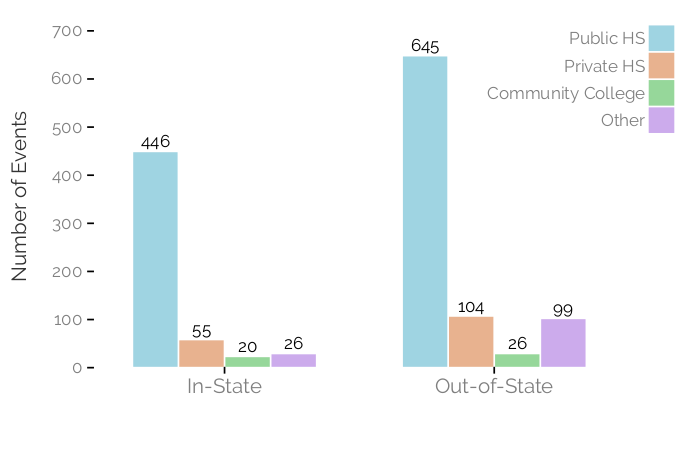
\includegraphics[width=0.45\textwidth, cfbox=Gray 0.4pt]{images/#2/visit_count}\hfill
    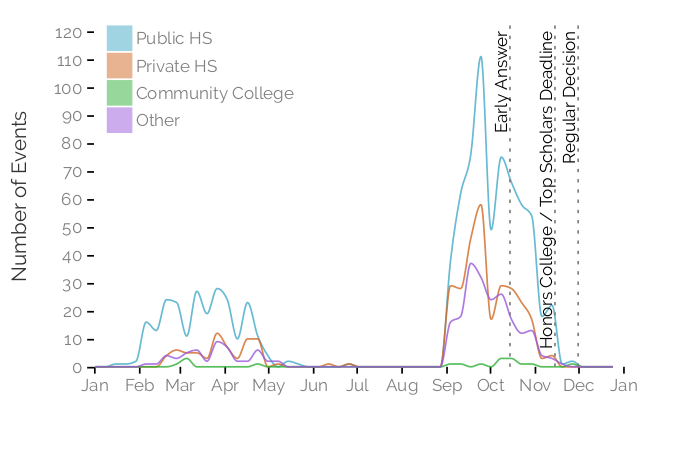
\includegraphics[width=0.45\textwidth, cfbox=Gray 0.4pt]{images/#2/timeline}

    \smallskip

    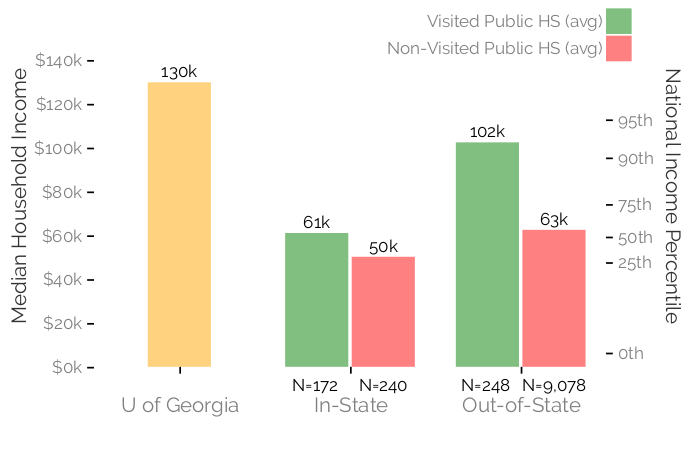
\includegraphics[width=0.45\textwidth, cfbox=Gray 0.4pt]{images/#2/median_income}\hfill
    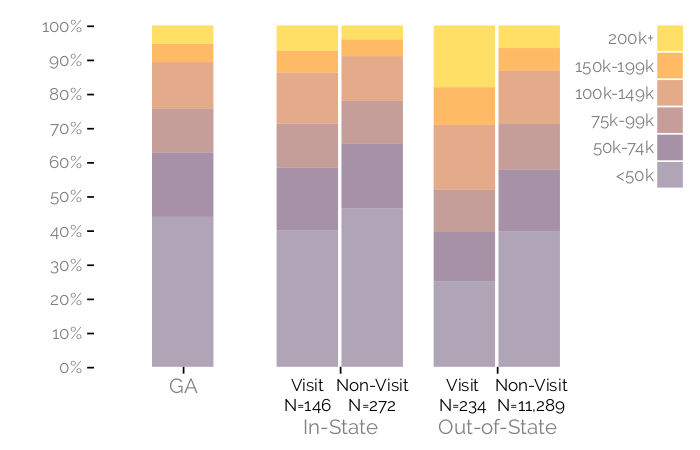
\includegraphics[width=0.45\textwidth, cfbox=Gray 0.4pt]{images/#2/income_band}

    \caption{\roboto\selectfont\textcolor{Gray}{\uppercase{#3}}}
    \label{fig:#4}

    \vspace{#1cm}
\end{figure*}
}

\newcommand{\addFigureCompare}[2] {  % Add row of 4 figures
\begin{figure}[!h]
    \vspace{0.45cm}
    \hspace{-1.6in}
    \color{Gray}\hdashrule{1.5\textwidth}{1pt}{1pt}\vspace{0.5cm}

    \centering

    \makebox[0.79\paperwidth][c]{\hspace{-3cm}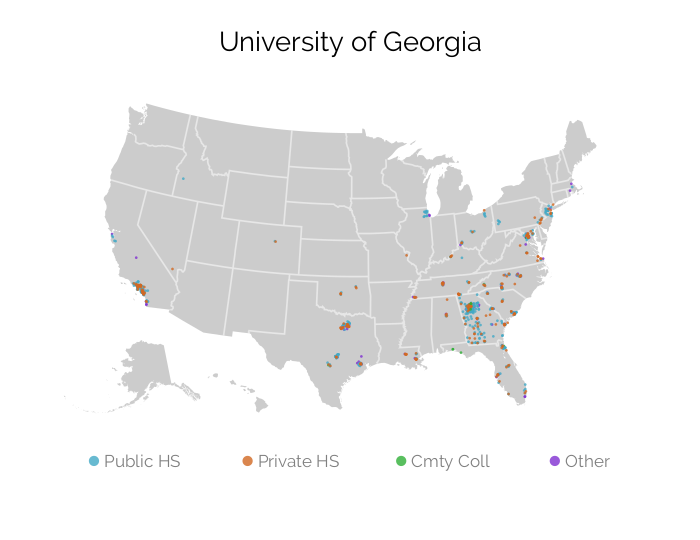
\includegraphics[width=0.2\paperwidth, cfbox=DarkGray 1pt]{images/139959/titled_map}\hfill
    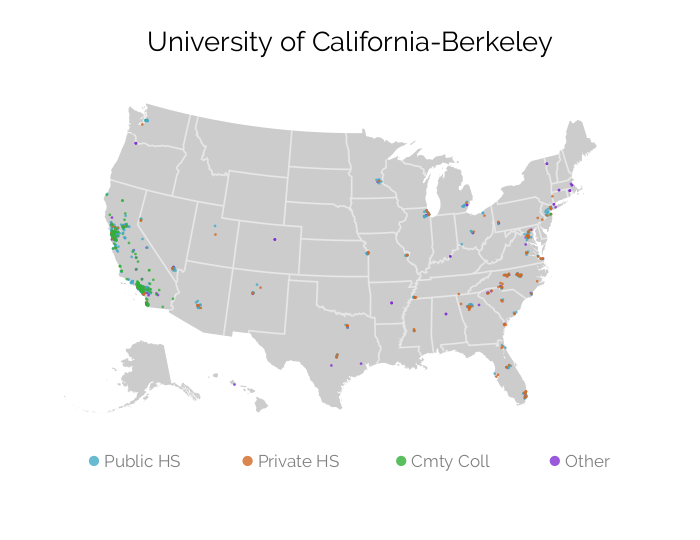
\includegraphics[width=0.2\paperwidth, cfbox=DarkGray 1pt]{images/110635/titled_map}\hfill
    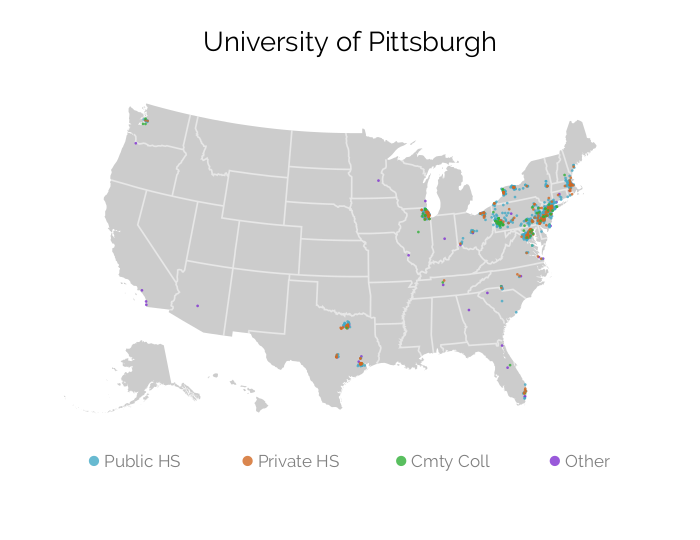
\includegraphics[width=0.2\paperwidth, cfbox=DarkGray 1pt]{images/215293/titled_map}\hfill
    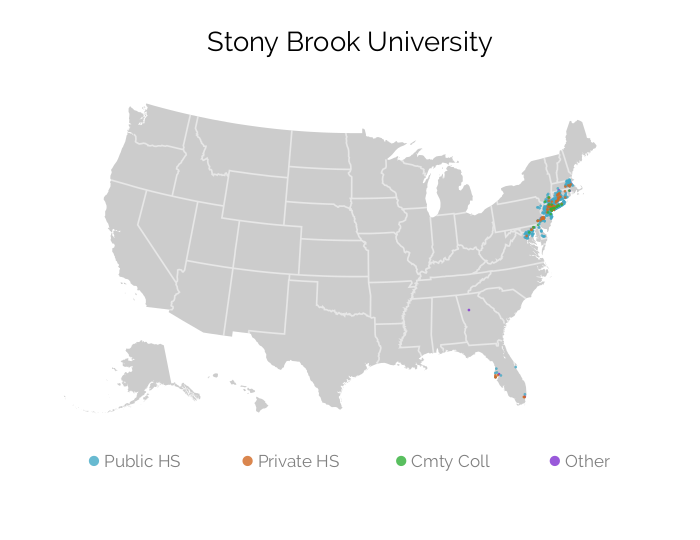
\includegraphics[width=0.2\paperwidth, cfbox=DarkGray 1pt]{images/196097/titled_map}}

    \caption{\roboto\selectfont\textcolor{Gray}{\uppercase{#1}}}
    \label{fig:#2}
    \makebox[0.79\paperwidth][c]{\hdashrule{1.5\paperwidth}{1pt}{1pt}}

\end{figure}
\vspace{0.45cm}
}


% Tables ~~~~

\usepackage{rotating}
\usepackage{multirow}
\usepackage[table]{xcolor}

\newcommand{\addTable}[4][p] {  % Add Table
\begin{table*}[t] % t or b

    \ifnum\pdfstrcmp{#1}{l}=0
      \begin{sideways}
    \fi

    \centering

    \begingroup
      \fontsize{8pt}{10pt}\selectfont
      \input{tables/#2.tex}
    \endgroup

    \ifnum\pdfstrcmp{#1}{l}=0
      \end{sideways}
    \fi

    \vspace{0.2cm}
    \caption{\roboto\selectfont\textcolor{Gray}{\uppercase{#3}}}
    \label{tbl:#4}

\end{table*}
}
